
\section{Électroaimant}

\subsection{Chargeur du condensateur}

%%% Image chargeur
  \begin{figure}[ht]
    \centering
    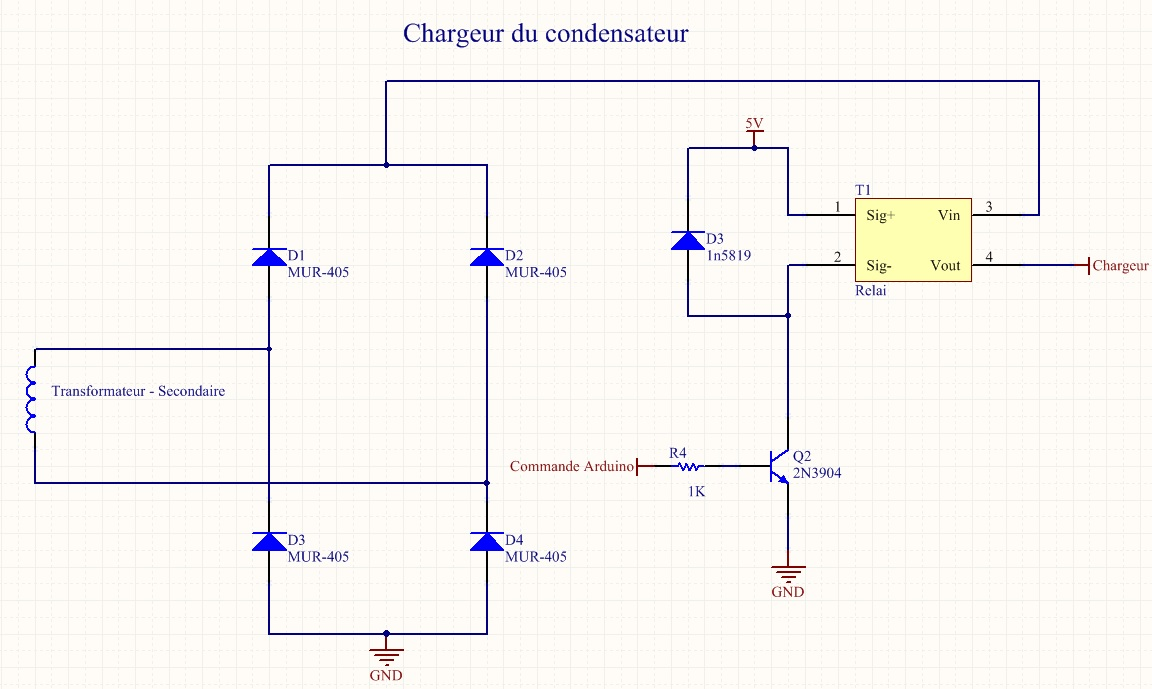
\includegraphics[scale=0.4]{resources/chargeur.jpg}
    \caption{Schéma électronique du chargeur du condensateur}
    \label{fig:chargeur}
  \end{figure}

La première étape de la charge du condensateur telle que représentée sur la figure \ref{fig:chargeur} est le redressage.
On utilise un pont diodes pour redresser notre signal alternatif.
Par la suite, on entre ce signal dans notre relai qui relie le pont de diodes aux condensateurs.
Il s'agit de la pièce T1 sur le schéma.
L'activation du relai est commandé par le arduino qui envoie un signal 0-5 volts dans la base du transistor qui \textit{drive} la bobine qui permet de
fermer l'interrupteur du relai.
Lorsqu'on active le relai, celui-ci devient un court-circuit et puisque notre charge est inductive on charge à la vitesse maximale
que le circuit d'induction peut fournir la puissance. En effet, si on applique une tension continue aux bornes d'un condensateur,
on obtient un théorie un courant infini. Cependant, ici le courant est limité par le circuit d'induction.

\subsection{Électroaimant et voltage des condensateurs}

%%% image electroaimant_probage
  \begin{figure}[ht]
    \centering
    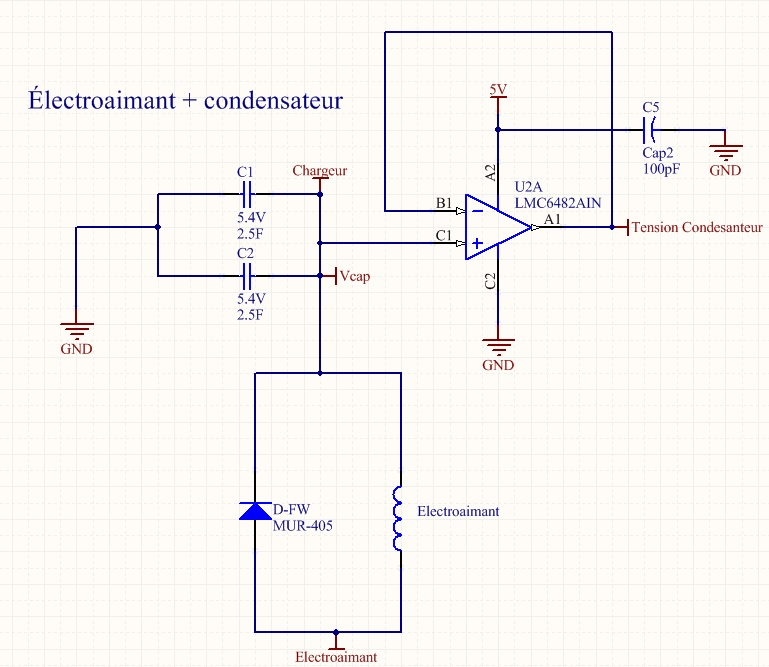
\includegraphics[scale=0.3]{resources/electroaimant_probage.jpg}
    \caption{Schéma électronique de l'électroaimant}
    \label{fig:electroaimant}
  \end{figure}

On observe sur la figure \ref{fig:electroaimant} la banque de condensateur qui sert à alimenter notre électroaimant.
On mesure la tension des condensateurs avec un amplificateur opérationnel Rail-to-rail en mode suiveur.
La sortie de cette amplificateur est fournit au convertisseur analogique-numérique du Arduino.
On a mis un condensateur de découplage sur son alimentation pour limiter le bruit sur l'alimentation.

\subsection{Régulation du courant dans la bobine}

%%% image regulation_current
  \begin{figure}[ht]
    \centering
    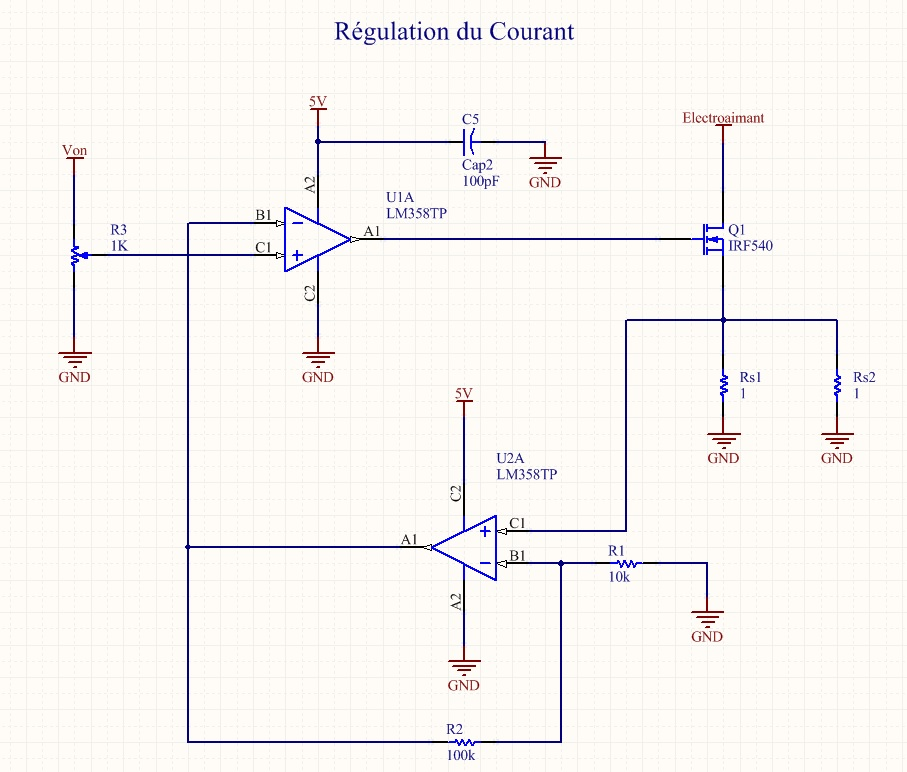
\includegraphics[scale=0.3]{resources/regulation_current.jpg}
    \caption{Schéma électronique de la régulation du courrant}
    \label{fig:reg_current}
  \end{figure}
Un régulateur analogique, tel que représenté à la figure \ref{fig:reg_current} est utilisé pour garder le courant constant dans la bobine.
Pour ce faire, une source courant est créée avec un MOSFET, dont la consigne provient de l'erreur entre la commande et le courant mesuré dans le canal
du MOSFET qui a été amplifié par une amplificateur en mode non-inverseur. La consigne est Von provient du arduino qui peut allumer ou fermer l'électroaimant.
Encore ici, on a mis un condensateur de découplage sur l'alimentation de l'amplificateur.

\subsection{Décharge du condensateur}

%%% decharge
  \begin{figure}[ht]
    \centering
    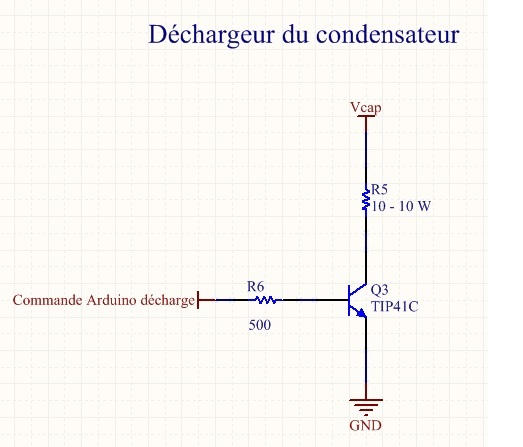
\includegraphics[scale=0.5]{resources/decharge.jpg}
    \caption{Schéma électronique de la décharge du condensateur}
    \label{fig:decharge}
  \end{figure}

Pour vider la charge dans le condensateur. On procède simplement en utilisant un transistor qui permet de vider la charge du condensateur
dans une résistance de puissance, tel que sur le shéma de la figure \ref{fig:decharge}.
